% 
% Annual Cognitive Science Conference
% Sample LaTeX Paper -- Proceedings Format
% 

% Original : Ashwin Ram (ashwin@cc.gatech.edu)       04/01/1994
% Modified : Johanna Moore (jmoore@cs.pitt.edu)      03/17/1995
% Modified : David Noelle (noelle@ucsd.edu)          03/15/1996
% Modified : Pat Langley (langley@cs.stanford.edu)   01/26/1997
% Latex2e corrections by Ramin Charles Nakisa        01/28/1997 
% Modified : Tina Eliassi-Rad (eliassi@cs.wisc.edu)  01/31/1998
% Modified : Trisha Yannuzzi (trisha@ircs.upenn.edu) 12/28/1999 (in process)
% Modified : Mary Ellen Foster (M.E.Foster@ed.ac.uk) 12/11/2000
% Modified : Ken Forbus                              01/23/2004
% Modified : Eli M. Silk (esilk@pitt.edu)            05/24/2005
% Modified : Niels Taatgen (taatgen@cmu.edu)         10/24/2006
% Modified : David Noelle (dnoelle@ucmerced.edu)     11/19/2014
% Modified : Roger Levy (rplevy@mit.edu)     12/31/2018



%% Change "letterpaper" in the following line to "a4paper" if you must.

\documentclass[10pt,letterpaper]{article}

\usepackage{cogsci}
\usepackage{color}
\usepackage{graphicx}

%\cogscifinalcopy % Uncomment this line for the final submission 

\usepackage{pslatex}
\usepackage{apacite}
\usepackage{float} % Roger Levy added this and changed figure/table
                   % placement to [H] for conformity to Word template,
                   % though floating tables and figures to top is
                   % still generally recommended!
\usepackage{booktabs}
\usepackage{chngpage}

%\usepackage{gb4e}
\usepackage{lingmacros}

%\usepackage[none]{hyphenat} % Sometimes it can be useful to turn off
%hyphenation for purposes such as spell checking of the resulting
%PDF.  Uncomment this block to turn off hyphenation.

\definecolor{Orange}{RGB}{255,140,0}
\newcommand{\ek}[1]{\textcolor{Orange}{[ek: #1]}} 

\definecolor{Green}{RGB}{0,255,0}
\newcommand{\jd}[1]{\textcolor{Green}{[jd: #1]}}

\setlength\titlebox{6cm}
% You can expand the titlebox if you need extra space
% to show all the authors. Please do not make the titlebox
% smaller than 4.5cm (the original size).
%%If you do, we reserve the right to require you to change it back in
%%the camera-ready version, which could interfere with the timely
%%appearance of your paper in the Proceedings.



\title{Effect of Reproduction on the Suspect Presentation in Crime Stories}
 
\author{{\large \bf Elisa Kreiss (ekreiss@stanford.edu)} \\
  Department of Linguistics, Margaret Jacks Hall, Bldg. 460 \\
  Stanford, CA 94305 USA
  \AND {\large \bf Michael Franke (...)} \\
  Department of Cognitive Science, Wachsbleiche 27 \\
  Osnabrück, Lower Saxony 49090 Germany
  \AND {\large \bf Judith Degen (jdegen@stanford.edu)} \\
  Department of Linguistics, Margaret Jacks Hall, Bldg. 460 \\
  Stanford, CA 94305 USA}


\begin{document}

\maketitle


\begin{abstract}
Include no author information in the initial submission, to facilitate
blind review.  The abstract should be one paragraph, indented 1/8~inch on both sides,
in 9~point font with single spacing. The heading ``{\bf Abstract}''
should be 10~point, bold, centered, with one line of space below
it. This one-paragraph abstract section is required only for standard
six page proceedings papers. Following the abstract should be a blank
line, followed by the header ``{\bf Keywords:}'' and a list of
descriptive keywords separated by semicolons, all in 9~point font, as
shown below.

\textbf{Keywords:} 
iterated narration; transmission chains; crime stories; suspect; guilt
\end{abstract}

\ek{General notes: make up your mind about generations vs. reproduction; original stories vs. seeds; stories vs. storytype vs. condition,...}\\
\section{Introduction}
One of the central goals in language use is the exchange of information. We obtain new information by reading the newspaper, or listening to the radio or a friend. We can use this newly acquired knowledge and communicate it to other people in our environment. In its simplified linear form, we know this transmission phenomenon as the game of Telephone. The first person whispers a sentence to their neighbor, who in turn has to pass it on to the next person, and so on. After several iterations, the last person in the chain announces the sentence which they ended up with. To everyone's amusement, we often find that this final sentence differs remarkably from the initial one. This simple game nicely exemplifies the information loss and distortion that is associated with repeated exposure and reproduction of information.\\
\cite{Bartlett:1932} first introduces this methodology of transmission chains, i.e., chains of reproductions, as a scientific method. In his book "Remembering" \cite{Bartlett:1932}, he presents a series of transmission chain studies, using stories such as Native American tales or sport reports for reproduction. Bartlett observes a significant information loss of the stories over generations of reproductions and that the content of the stories changes \ek{en par} with the reproducer's prior knowledge. Bartlett used these observations as a foundation for his theory that memory retrieval involves a process of reconstruction. \\
In recent years, the transmission chain method received a revival in the scientific community. \ek{Mesoudi and Whiten} extend Bartlett's generalization hypothesis by using script theory to show that with each iteration, the described events become increasingly abstract. Further research showed that \ek{gender stereotypes: Bangerter 2000, Kashima 2000; cognitive biases: Kalish 2007, Griffiths 2007/2008; Stubbersfield 2015/2017; Hills/Jagiello 2018}\\
In summary, we know that we use language and communication to exchange information, but we also know that the process of passing on information is flawed in very particular ways. Given their political relevance, we look at how crime stories change in a transmission chain and how this is influenced by seemingly weak and strong of evidence.\\

\begin{figure}[]
	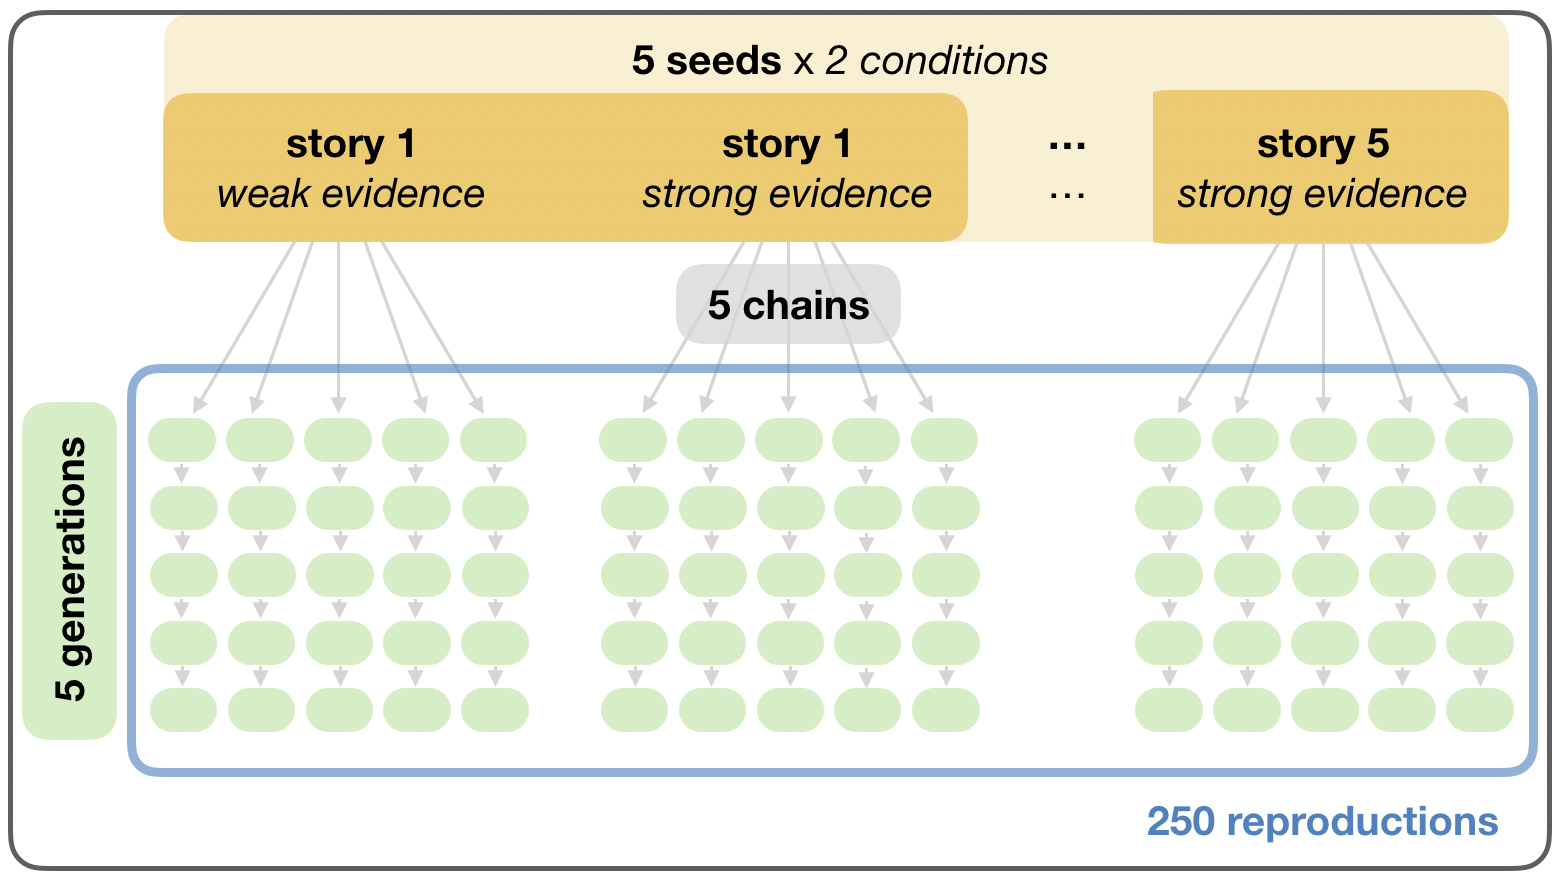
\includegraphics[width=0.48\textwidth]{graphs/corpus_overview.png}
	\caption{Overview of corpus of stories collected in Exp.~1.} 
	\label{fig:design}
\end{figure}

To investigate how crime stories evolve over iterations, we conducted two experiments. First we collected a corpus of reproductions for five crime stories, each addressing a different type of crime (e.g., animal smuggling, arson or sexual assault). Each story existed in a weak and a strong evidence condition. This manipulation has successfully been used by \cite{Van-Prooijen:2006} to uncover in- and out-group effects in guilt judgments. Similar to his study, the different conditions were achieved by changing the last sentence in the story which then either suggested strong or weak evidence. \\
We want to investigate how these stories develop in a transmission chain paradigm (as displayed in \ek{figure ref}).\\
To evaluate the stories' development, we conducted a second experiment which asked participants to answer questions about the suspect's guilt, the likelihood of conviction and other suspect, author and reader related questions. 


\section{Experiment 1: corpus collection}
\ek{transmission chain method}

\subsection{Methods}
74 Stanford students participated in this online study for course credit. 
We constructed five stories (\textit{seeds}) that marked the beginning of each reproduction chain.  Stories were written in the style of short news articles and followed a similar structure. They reported a crime or moral violation that occurred, the authorities' determination of  and search for the perpetrator(s), and  the possible punishment the suspects would face if found guilty. Furthermore, each of these five seed stories  occurred in one of two conditions: a \emph{weak evidence} and a \emph{strong evidence} condition. Evidence strength was manipulated in the final sentence of the story (see example seed in Table \ref{tab:examplestory}).

\begin{table*}
\caption{Example seed story in Exp.~1.}
\centering
\begin{tabular}{l l}
\toprule
\multicolumn{2}{c}{\jd{ELISA, INSERT EXAMPLE STORY HERE}}\\
\midrule
\jd{ELISA, INSERT STRONG EVIDENCE SENTENCE HERE} (\emph{strong evidence condition}) & \jd{ELISA, INSERT WEAK EVIDENCE SENTENCE HERE} (\emph{weak evidence condition})  \\
\bottomrule
\end{tabular}
\label{tab:examplestory}
\end{table*}

Each participant read and reproduced five stories (either only seed stories, a mix of seeds and reproductions from previous participants, or only reproductions). The assignment of the condition was random \jd{did a participant read either all weak or all strong evidence stories, or a mix?}. On each trial, participants first read a story. They were told to click the `Continue' button when they were confident they had internalized the story. Once they clicked the button, the story disappeared and they were asked to reproduce it freely in a text field.  Order of stories was randomized.

\subsection{Results}

Participants produced 370 stories. For each seed, we defined a complete chain as one that has 5 reproductions/generations. For subsequent analysis, we randomly selected 50 complete chains, evenly distributed across stories and conditions. This yielded a corpus of 250 reproductions (5 seeds in 2 conditions each with 5 complete chains each, see Figure \ref{fig:design}).

While the linguistic changes across generations as a function of the original evidence condition merit their own detailed analysis, we focus here on reporting only a few general features of the collected corpus, which we will subsequently use as predictors in the analyses of Exp.~2 below.

\textbf{Story length.} As shown in Figure \ref{fig:storylength}, the length of the stories decreased across generations ($\beta = XX$, $SE = XX$, $t = XX$, $p < XX$) \jd{elisa, fill in values}, replicating a well-known phenomenon in reproduction studies  \cite{Bartlett:1932}. While the original generation 0 seeds consisted on average of \jd{XX} words, that number dropped to \jd{XX} by generation 5. Examples of reproductions of the seed in Table \ref{tab:examplestory} from generation 1 and 5 are shown in (\ref{gen1}) and (\ref{gen5}) below.

%\begin{exe}
%	\ex\label{gen1} \jd{elisa, add story from gen 1 of seed in table 1}
%	\ex\label{gen5} \jd{elisa, add story from gen 5 of seed in table 1}
%\end{exe}

\enumsentence{\jd{elisa, add story from gen 1 of seed in table 1}.\label{gen1}}
\enumsentence{\jd{elisa, add story from gen 5 of seed in table 1}.\label{gen5}}

\begin{figure}[]
	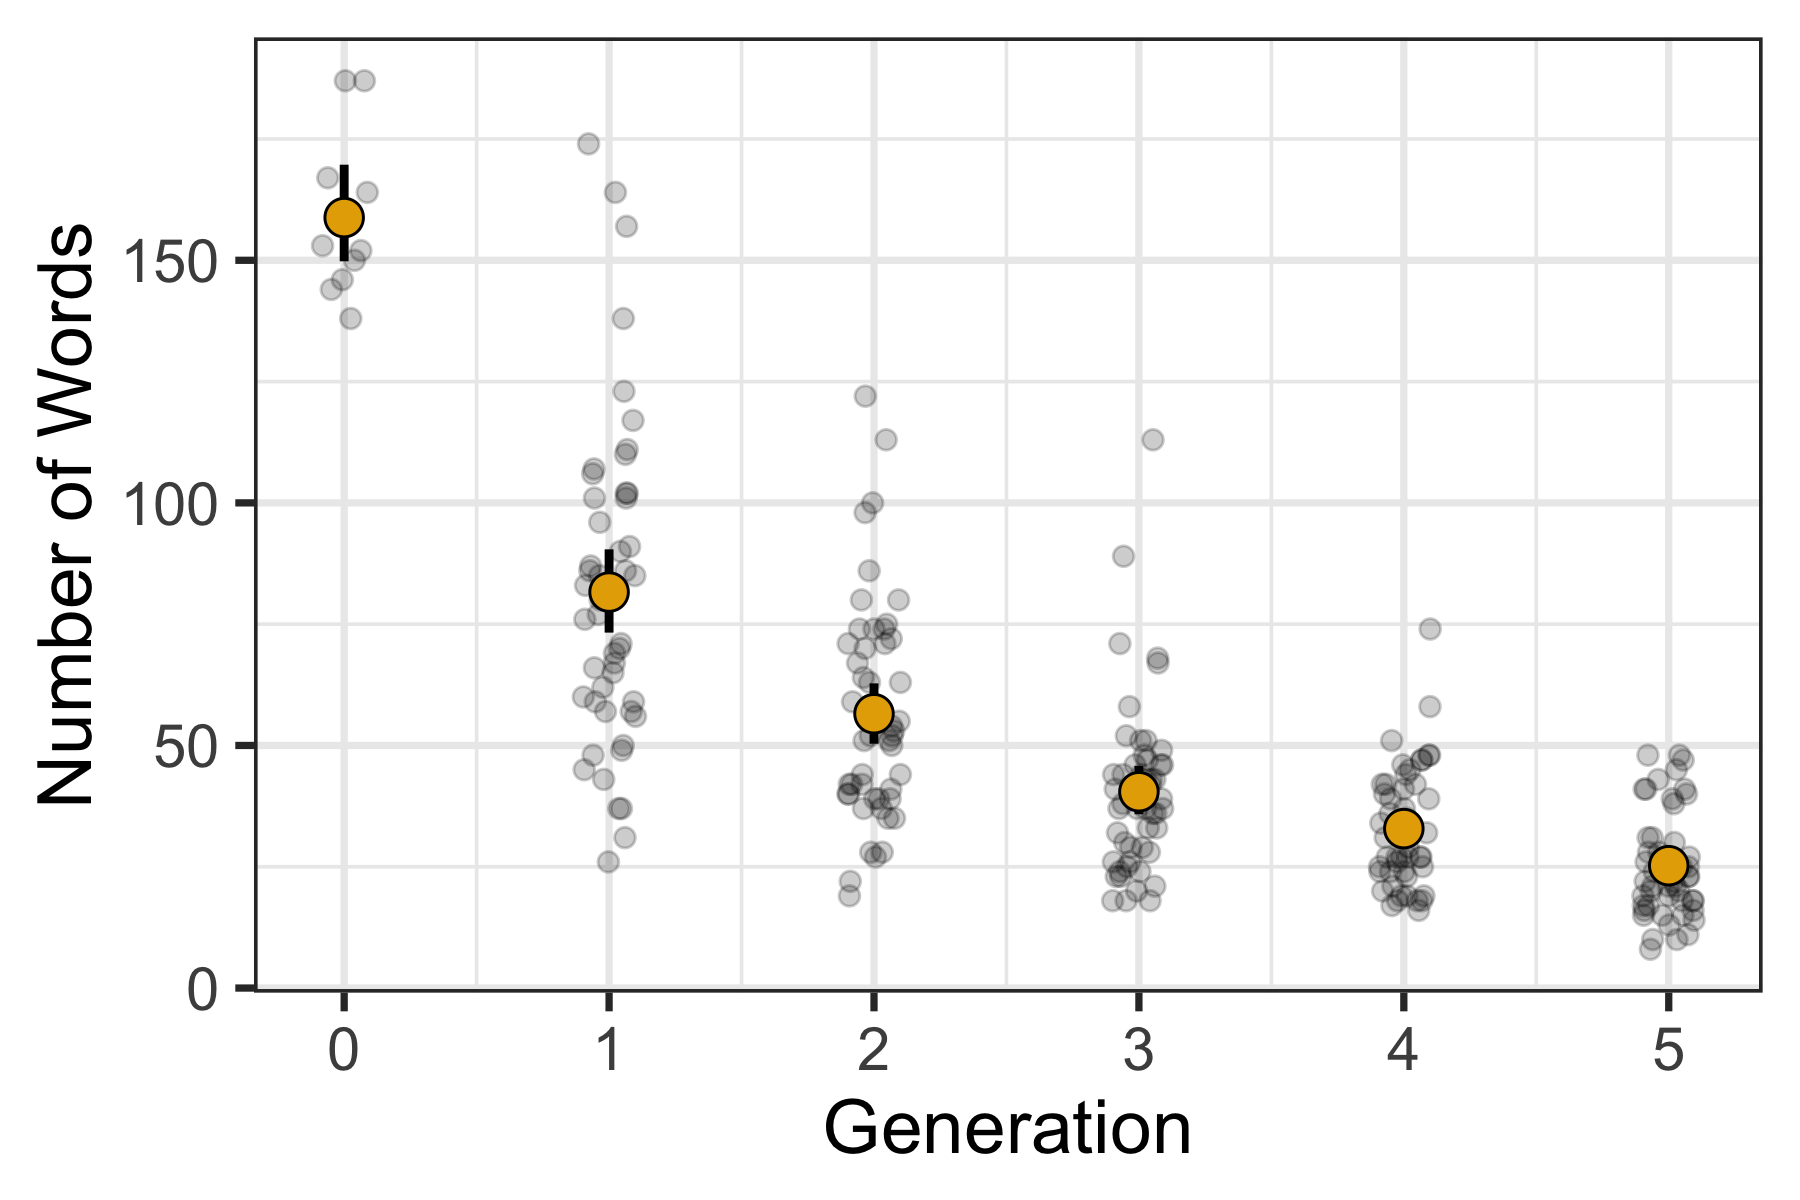
\includegraphics[width=0.48\textwidth]{graphs/corpus_length.png}
	\caption{Mean story length in number of words by generation. Error bars indicate bootstrapped 95\% CIs. Orange dots indicate generation mean, gray dots are individual stories. \jd{elisa, make sure that in all plots, only the first letter is capitalized (ie make "Words" lower case) and save the figures as pdf so they're not blurry}} 
	\label{fig:storylength}
\end{figure}

\textbf{Similarity of seeds and reproductions.} Of interest is the extent to which stories retain the gist or deviate from it. To assess the similarity of reproductions and their seed stories quantitatively, we computed the Jaccard distance between each reproduction and its generation 0 seed. Jaccard distance captures the amount of overlap between two stories in the following way: \jd{elisa, insert formula}, where XX is XX and XX is XX \jd{elisa, explain terms and say that we took words as the basic unit over which distance was computed}. Figure \ref{fig:jaccdistance} shows that $D_J$ increased across generations ($\beta = XX$, $SE = XX$, $t = XX$, $p < XX$) \jd{elisa, fill in values}. This is not surprising given that as story length decreases, $D_J$ between seed and any of its reproductions necessarily increases. However, $D_J$ increased more strongly than expected if the difference between stories was only due to the decrease in length, suggesting that information was lost across generations. This can also be observed qualitatively in the comparison of  the representative examples (\ref{gen1}) and (\ref{gen5})  above. \jd{ideally, the plot would include dots for the best possible  baseline in addition to the actual means.}

\begin{figure}[]
	%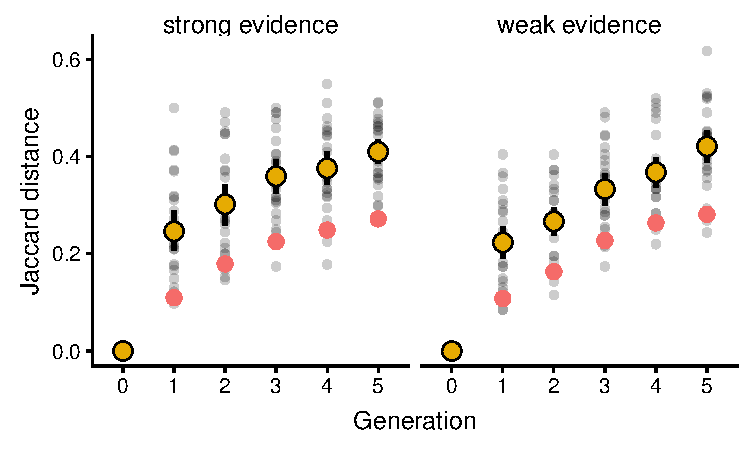
\includegraphics[width=0.48\textwidth]{graphs/jaccdistance}
	\caption{Mean Jaccard distance between seed and reproductions by generation in strong (left) and weak (right) evidence condition. Error bars indicate bootstrapped 95\% CIs. Orange dots indicate generation mean, gray dots are individual stories. \jd{elisa, make this plot analogous to fig 2 and uncomment the above when plot exists}} 
	\label{fig:jaccdistance}
\end{figure}

\section{Experiment 2: story ratings}
To evaluate the reproduction corpus, we obtained ratings for a variety of psychological variables to track their changes throughout the generations. We asked participants to answer questions about the suspect, the author, the reader and the evidence.

\subsection{Material}
The stories were taken from the corpus described in \ek{ref}.\\
In the questions, we asked about the evidence, the suspect's guilt and possible conviction, the reader's beliefs about the author and the reader's emotional connection to the story. \ek{a complete list of the questions can be found...} Overall, participants were asked eight questions of interest and four attention check questions. 

\subsection{Methods}
5392 participants were recruited over Amazon Mechanical Turk. Each participant read one story and answered twelve questions (including four attention checks). They indicated their response by moving a slider on a continuous scale. Each question was shown in isolation in a randomized order. Participants spent two to three minutes on this experiment and were paid 0.60ct (\$12-\$18 per hour). The story was visible throughout the experiment.

\subsection{Results}
\ek{...}\\
We excluded 12 participants because they completed the study multiple times and another 535 because they failed at least two of the attention check questions. This leaves us with 4573 participants (84.8\% of the original set). After the exclusion of the participants, each reproduction was rated on average by 17 subjects.

\begin{figure}[H]
	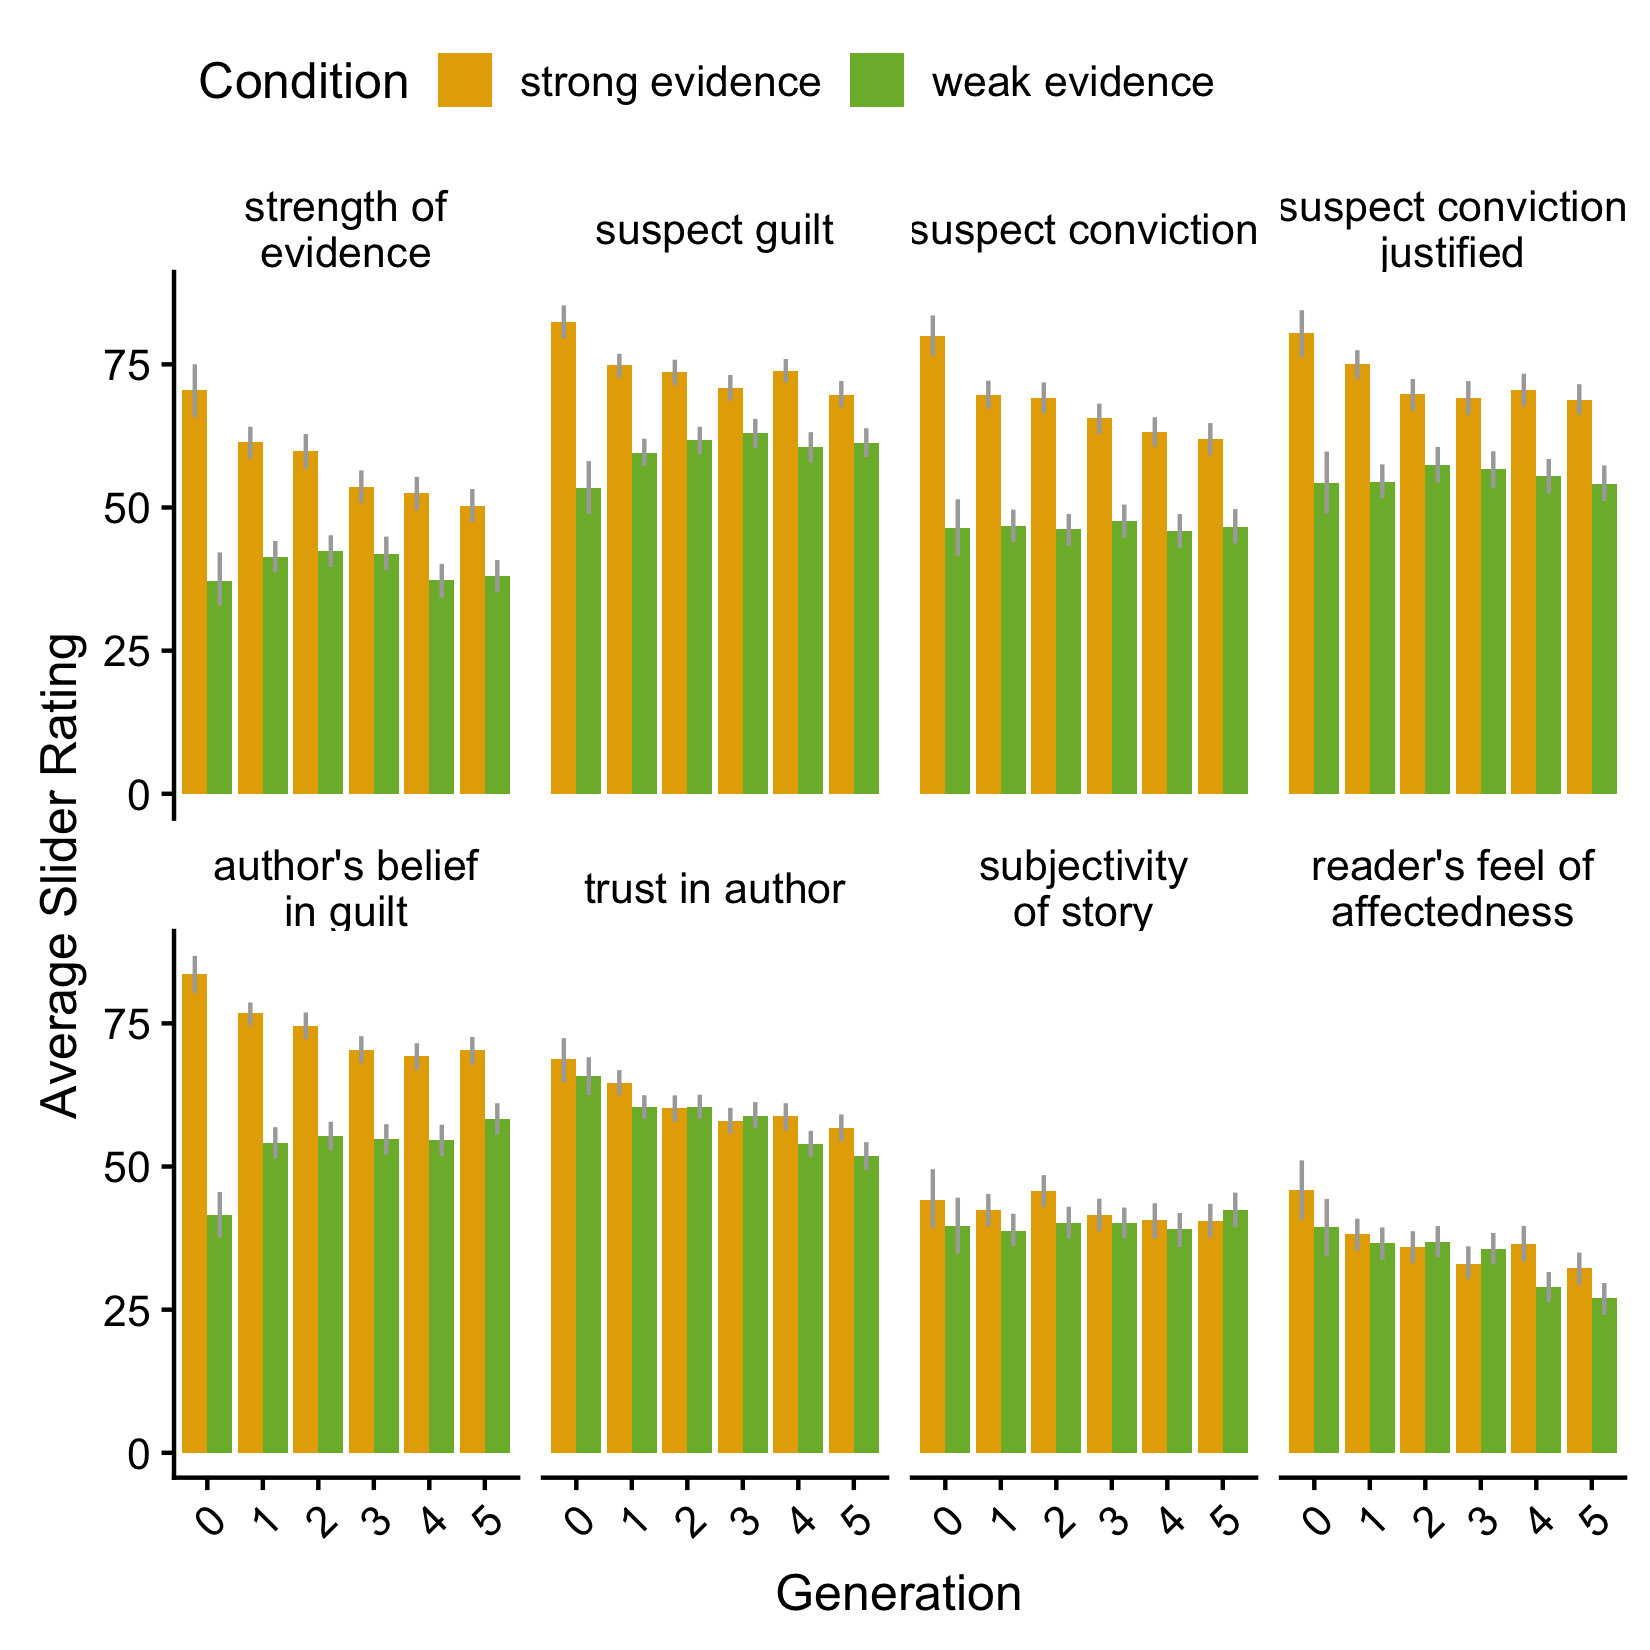
\includegraphics[width=0.48\textwidth]{graphs/subj_results_byquestion.png}
	\caption{Mean ratings  in strong (orange) and weak (green) evidence condition for each dimension (facets). \jd{elisa, put these all in one row, make the x-axis labels not slanted, and make it a two-column figure}} 
	\label{fig:exp2results}
\end{figure}



\section{Conclusion}

\section{Discussion}
\ek{discuss differences between stories iwth in- and out-group effects for smuggler and professor}


\bibliographystyle{apacite}

\setlength{\bibleftmargin}{.125in}
\setlength{\bibindent}{-\bibleftmargin}

\bibliography{cogsci_IN_bib}

\cleardoublepage
%\ek{TODO: condition title == facet labels}
\begin{adjustwidth}{-1in}{-1in}
	\begin{table}
		\centering
		\begin{tabular}{l r r l r r l r r l l l l}
			\toprule
			& \multicolumn{3}{c}{condition} & \multicolumn{3}{c}{generation} & \multicolumn{3}{c}{condition*generation} & \multicolumn{3}{c}{simple effects}\\
			& \multicolumn{1}{c}{$\beta$} & \multicolumn{1}{c}{SE} & \multicolumn{1}{c}{p} & \multicolumn{1}{c}{$\beta$} & \multicolumn{1}{c}{SE} & \multicolumn{1}{c}{p} & \multicolumn{1}{c}{$\beta$} & \multicolumn{1}{c}{SE} & \multicolumn{1}{c}{p} & \multicolumn{1}{c}{weak} & \multicolumn{1}{c}{str*gen} & \multicolumn{1}{c}{we*gen}\\
			\midrule
			evidence                  & -23.25 & 4.09 & $<$0.0001*** & -3.42 & 0.89 & $<$0.001*** & 2.59  & 1.26 & $<$0.05*  & *** & *** & \\
			suspect guilt          & -17.28  & 3.40 & $<$0.0001*** & -1.34 & 0.74 & $<$0.08           & 1.90  & 1.05 & $<$0.08 & *** & . & \\
			conviction               & -27.01 & 4.15  & $<$0.0001*** & -2.79 & 0.90 & $<$0.01**     & 2.74  & 1.28 & $<$0.05*  & *** & ** & \\
			convicJustified       & -19.02 & 4.35 & $<$0.0001***  & -1.69 & 0.95 & $<$0.08           & 1.43 & 1.34 & $<$0.29   & *** & . &  \\
			author belief            & -27.53 & 3.72 & $<$0.0001***  & -2.14 & 0.81 & $<$0.01**      & 3.42  & 1.15 & $<$0.01** & *** & ** & \\
			author trust            & -0.82   & 2.25 & $<$0.72           & -1.94 & 0.49 & $<$0.001*** & -0.54 & 0.70 & $<$0.44   & & *** & *** \\
			story subjectivity     & -6.12   & 2.21 & $<$0.01**          & -0.86 & 0.49 & $<$0.08         & 1.40   & 0.69 & $<$0.05* & ** & . & \\
			reader emotion        & 0.85   & 2.99 & $<$0.78            & -1.49 & 0.65 & $<$0.05*     & -1.11  & 0.92 & $<$0.24  & * & *** & 
			%			\bottomrule
		\end{tabular}
		\caption{lmer(suspectconvictionJustified ~ generation * condition + (1|storyreproduction), data=dfmodel); high correlation of fixed effects}
		\label{tab:generationmodel}
	\end{table}
\end{adjustwidth}

%\begin{adjustwidth}{-1in}{-1in}
%	\begin{table}
%		\centering
%		\begin{tabular}{l r r l r r l r r l}
%			\toprule
%			& \multicolumn{3}{c}{condition} & \multicolumn{3}{c}{generation} & \multicolumn{3}{c}{condition*generation}\\
%			& \multicolumn{1}{c}{$\beta$} & \multicolumn{1}{c}{SE} & \multicolumn{1}{c}{p} & \multicolumn{1}{c}{$\beta$} & \multicolumn{1}{c}{SE} & \multicolumn{1}{c}{p} & \multicolumn{1}{c}{$\beta$} & \multicolumn{1}{c}{SE} & \multicolumn{1}{c}{p}\\
%			\midrule
%			evidence                              & -23.25 & 4.09 & $<$0.0001*** & -3.42 & 0.89 & $<$0.001*** & 2.59  & 1.26 & $<$0.05*  \\
%			suspect committedCrime    & -17.28  & 3.40 & $<$0.0001*** & -1.34 & 0.74 & $<$0.08           & 1.90  & 1.05 & $<$0.08  \\
%			suspect conviction              & -27.01 & 4.15  & $<$0.0001*** & -2.79 & 0.90 & $<$0.01**     & 2.74  & 1.28 & $<$0.05*  \\
%			suspect convictionJustified & -19.02 & 4.35 & $<$0.0001***  & -1.69 & 0.95 & $<$0.08           & 1.43 & 1.34 & $<$0.29    \\
%			author belief                        & -27.53 & 3.72 & $<$0.0001***  & -2.14 & 0.81 & $<$0.01**      & 3.42  & 1.15 & $<$0.01** \\
%			author trust                          & -0.82   & 2.25 & $<$0.72           & -1.94 & 0.49 & $<$0.001*** & -0.54 & 0.70 & $<$0.44   \\
%			story subjectivity                 & -6.12   & 2.21 & $<$0.01**          & -0.86 & 0.49 & $<$0.08         & 1.40   & 0.69 & $<$0.05*  \\
%			reader emotion                    & 0.85   & 2.99 & $<$0.78            & -1.49 & 0.65 & $<$0.05*     & -1.11  & 0.92 & $<$0.24  
%			%			\bottomrule
%		\end{tabular}
%		\caption{some caption}
%		\label{tab:generationmodel}
%	\end{table}
%\end{adjustwidth}

\begin{adjustwidth}{-1in}{-1in}
	\begin{table}
		\centering
		\begin{tabular}{l r r l r r l r r l}
			\toprule
			& \multicolumn{3}{c}{condition} & \multicolumn{3}{c}{distance} & \multicolumn{3}{c}{condition*distance} \\
			& \multicolumn{1}{c}{$\beta$} & \multicolumn{1}{c}{SE} & \multicolumn{1}{c}{p} & \multicolumn{1}{c}{$\beta$} & \multicolumn{1}{c}{SE} & \multicolumn{1}{c}{p} & \multicolumn{1}{c}{$\beta$} & \multicolumn{1}{c}{SE} & \multicolumn{1}{c}{p}\\
			\midrule
			evidence                              & -24.90 & 5.24 & $<$0.0001*** & -36.49 & 10.92 & $<$0.001*** & 27.75  & 15.41 & $<$0.08  \\
			suspect committedCrime    & -20.12  & 4.32 & $<$0.0001*** & -14.94 & 9.00 & $<$0.10          & 26.15  & 12.71 & $<$0.05*  \\
			suspect conviction              & -31.87 & 5.26  & $<$0.0001*** & -36.83 & 10.96 & $<$0.001***  & 39.48  & 15.47 & $<$0.05*  \\
			suspect convictionJustified & -21.181 & 5.54 & $<$0.001***  & -21.42 & 11.55 & $<$0.07        & 19.35  & 16.30 & $<$0.24    \\
			author belief                        & -29.90 & 4.74 & $<$0.0001***  & -9.01 & 9.87 & $<$0.37      & 39.02  & 13.94 & $<$0.01** \\
			author trust                          & -1.19   & 2.83 & $<$0.68             & -24.73 & 5.91 & $<$0.001*** & -4.93 & 8.36 & $<$0.56   \\
			story subjectivity                 & -6.12   & 2.77 & $<$0.05*          & -5.05 & 5.79 & $<$0.39         & 12.77   & 8.22 & $<$0.13  \\
			reader emotion                    & 0.54   & 3.70 & $<$0.89             & -25.34 & 7.72 & $<$0.01**     & -10.44  & 10.93 & $<$0.35  
			%			\bottomrule
		\end{tabular}
		\caption{lmer(suspectconvictionJustified ~ sim * condition + (1|storyreproduction), data=dfmodel); high correlation of fixed effects}
		\label{tab:distancemodel}
	\end{table}
\end{adjustwidth}

\cleardoublepage

\begin{adjustwidth}{-1in}{-1in}
	\begin{table}
		\centering
		\begin{tabular}{l r r l r r l r r l}
			\toprule
			& \multicolumn{3}{c}{condition} & \multicolumn{3}{c}{hedgesprop} & \multicolumn{3}{c}{condition*hedgesprop} \\
			& \multicolumn{1}{c}{$\beta$} & \multicolumn{1}{c}{SE} & \multicolumn{1}{c}{p} & \multicolumn{1}{c}{$\beta$} & \multicolumn{1}{c}{SE} & \multicolumn{1}{c}{p} & \multicolumn{1}{c}{$\beta$} & \multicolumn{1}{c}{SE} & \multicolumn{1}{c}{p}\\
			\midrule
			evidence                              & -15.74 & 1.95 & $<$0.0001*** & 101.20 & 56.55 & $<$0.08      & -119.12  & 82.37 & $<$0.15  \\
			suspect committedCrime    & -11.93  & 1.59 & $<$0.0001*** & 43.01 & 45.98 & $<$0.36      & -118.58  & 66.97 & $<$0.08  \\
			suspect conviction              & -19.10 & 1.96  & $<$0.0001*** & 102.66 & 56.65 & $<$0.08  & -132.10  & 82.50 & $<$0.12  \\
			suspect convictionJustified & -14.94 & 2.04 & $<$0.0001***  & 30.91 & 59.10 & $<$0.7        & -70.91  & 86.08 & $<$0.42    \\
			author belief                        & -17.91 & 1.75 & $<$0.0001***  & 54.69 & 50.54 & $<$0.29      & -188.17  & 73.61 & $<$0.05* \\
			author trust                          & -2.16   & 1.13 & $<$0.06            & 46.60 & 32.70 & $<$0.16     & 27.80 & 47.74 & $<$0.57   \\
			story subjectivity                 & -2.22   & 1.06 & $<$0.05*          & 6.10 & 30.61 & $<$0.85         & -45.08  & 44.85 & $<$0.32  \\
			reader emotion                    & -2.25   & 1.46 & $<$0.13             & -7.18 & 42.26 & $<$0.87     & 49.49  & 61.67 & $<$0.43  
			%			\bottomrule
		\end{tabular}
		\caption{lmer(suspectconvictionJustified ~ hedgesprop * condition + (1|storyreproduction), data=dfmodel); hedges is centered; hedges = c("allegedly", "possibly", "maybe", "probably", "if", "around", "over", "nearly", "almost", "approximately", "vaguely", "up to", "roughly", "mainly", "kind of", "sort of", "kinda", "sorta", "about", "supposedly", "seem", "tend", "look like", "looks like", "appear to be", "think", "believe", "doubt", "be sure", "indicate", "suggest", "assume", "might", "perhaps", "possibility")}
		\label{tab:hedgemodel}
	\end{table}
\end{adjustwidth}

%
%
%\section{General Formatting Instructions}
%
%The entire content of a paper (including figures, references, and anything else) can be no longer than six pages in the \textbf{initial submission}. In the \textbf{final submission}, the text of the paper, including an author line, must fit on six pages. Up to one additional page can be used for acknowledgements and references.
%
%The text of the paper should be formatted in two columns with an
%overall width of 7 inches (17.8 cm) and length of 9.25 inches (23.5
%cm), with 0.25 inches between the columns. Leave two line spaces
%between the last author listed and the text of the paper; the text of
%the paper (starting with the abstract) should begin no less than 2.75 inches below the top of the
%page. The left margin should be 0.75 inches and the top margin should
%be 1 inch.  \textbf{The right and bottom margins will depend on
%  whether you use U.S. letter or A4 paper, so you must be sure to
%  measure the width of the printed text.} Use 10~point Times Roman
%with 12~point vertical spacing, unless otherwise specified.
%
%The title should be in 14~point bold font, centered. The title should
%be formatted with initial caps (the first letter of content words
%capitalized and the rest lower case). In the initial submission, the
%phrase ``Anonymous CogSci submission'' should appear below the title,
%centered, in 11~point bold font.  In the final submission, each
%author's name should appear on a separate line, 11~point bold, and
%centered, with the author's email address in parentheses. Under each
%author's name list the author's affiliation and postal address in
%ordinary 10~point type.
%
%Indent the first line of each paragraph by 1/8~inch (except for the
%first paragraph of a new section). Do not add extra vertical space
%between paragraphs.
%
%
%\section{First Level Headings}
%
%First level headings should be in 12~point, initial caps, bold and
%centered. Leave one line space above the heading and 1/4~line space
%below the heading.
%
%
%\subsection{Second Level Headings}
%
%Second level headings should be 11~point, initial caps, bold, and
%flush left. Leave one line space above the heading and 1/4~line
%space below the heading.
%
%
%\subsubsection{Third Level Headings}
%
%Third level headings should be 10~point, initial caps, bold, and flush
%left. Leave one line space above the heading, but no space after the
%heading.
%
%
%\section{Formalities, Footnotes, and Floats}
%
%Use standard APA citation format. Citations within the text should
%include the author's last name and year. If the authors' names are
%included in the sentence, place only the year in parentheses, as in
%\citeA{NewellSimon1972a}, but otherwise place the entire reference in
%parentheses with the authors and year separated by a comma
%\cite{NewellSimon1972a}. List multiple references alphabetically and
%separate them by semicolons
%\cite{ChalnickBillman1988a,NewellSimon1972a}. Use the
%``et~al.'' construction only after listing all the authors to a
%publication in an earlier reference and for citations with four or
%more authors.
%
%
%\subsection{Footnotes}
%
%Indicate footnotes with a number\footnote{Sample of the first
%footnote.} in the text. Place the footnotes in 9~point font at the
%bottom of the column on which they appear. Precede the footnote block
%with a horizontal rule.\footnote{Sample of the second footnote.}
%
%
%\subsection{Tables}
%
%Number tables consecutively. Place the table number and title (in
%10~point) above the table with one line space above the caption and
%one line space below it, as in Table~\ref{sample-table}. You may float
%tables to the top or bottom of a column, and you may set wide tables across
%both columns.
%
%\begin{table}[H]
%\begin{center} 
%\caption{Sample table title.} 
%\label{sample-table} 
%\vskip 0.12in
%\begin{tabular}{ll} 
%\hline
%Error type    &  Example \\
%\hline
%Take smaller        &   63 - 44 = 21 \\
%Always borrow~~~~   &   96 - 42 = 34 \\
%0 - N = N           &   70 - 47 = 37 \\
%0 - N = 0           &   70 - 47 = 30 \\
%\hline
%\end{tabular} 
%\end{center} 
%\end{table}
%
%
%\subsection{Figures}
%
%All artwork must be very dark for purposes of reproduction and should
%not be hand drawn. Number figures sequentially, placing the figure
%number and caption, in 10~point, after the figure with one line space
%above the caption and one line space below it, as in
%Figure~\ref{sample-figure}. If necessary, leave extra white space at
%the bottom of the page to avoid splitting the figure and figure
%caption. You may float figures to the top or bottom of a column, and
%you may set wide figures across both columns.
%
%\begin{figure}[H]
%\begin{center}
%\fbox{CoGNiTiVe ScIeNcE}
%\end{center}
%\caption{This is a figure.} 
%\label{sample-figure}
%\end{figure}
%
%
%\section{Acknowledgments}
%
%In the \textbf{initial submission}, please \textbf{do not include
%  acknowledgements}, to preserve anonymity.  In the \textbf{final submission},
%place acknowledgments (including funding information) in a section \textbf{at
%the end of the paper}.
%
%
%\section{References Instructions}
%
%Follow the APA Publication Manual for citation format, both within the
%text and in the reference list, with the following exceptions: (a) do
%not cite the page numbers of any book, including chapters in edited
%volumes; (b) use the same format for unpublished references as for
%published ones. Alphabetize references by the surnames of the authors,
%with single author entries preceding multiple author entries. Order
%references by the same authors by the year of publication, with the
%earliest first.
%
%Use a first level section heading, ``{\bf References}'', as shown
%below. Use a hanging indent style, with the first line of the
%reference flush against the left margin and subsequent lines indented
%by 1/8~inch. Below are example references for a conference paper, book
%chapter, journal article, dissertation, book, technical report, and
%edited volume, respectively.
%
%\nocite{ChalnickBillman1988a}
%\nocite{Feigenbaum1963a}
%\nocite{Hill1983a}
%\nocite{OhlssonLangley1985a}
%% \nocite{Lewis1978a}
%\nocite{Matlock2001}
%\nocite{NewellSimon1972a}
%\nocite{ShragerLangley1990a}





\end{document}
